\documentclass[a4paper,11pt]{article}
\usepackage[separate-uncertainty]{siunitx}
\usepackage[siunitx]{gnuplottex}
\usepackage{csvsimple}
\usepackage{booktabs}
\usepackage[margin=1in,tmargin=1in]{geometry}
\usepackage[square,numbers]{natbib}
\usepackage{parskip}
\usepackage{url}
\usepackage{fancyhdr}

\pagestyle{fancy}
\fancyhf{}
\lhead{\url{https://github.com/elterminad0r/physics/tree/master/thermal_cap}}

\begin{document}

Figure \ref{fig:graph} shows the graph of temperature against time. Some of the
various calculated
\footnote{\url{https://github.com/elterminad0r/physics/tree/master/thermal_cap/analyse.r}}
and recorded values are listed in table \ref{tab:values}.

Using the additive model in the graph, I calculated $c$ as
\SI{0.45}{\joule\per\gram}.

This value of $c$ agrees with various other values I've found:

\begin{itemize}
\item $c = \SI{0.460548}{\joule\per\gram}$ \cite{EngineersEdge}
\item $c = \SI{0.450}{\joule\per\gram}$ \cite{DeLeon}
\item $c = \SI{0.444}{\joule\per\gram}$ \cite{Stretton}
\end{itemize}

\begin{figure}[h]
\begin{center}
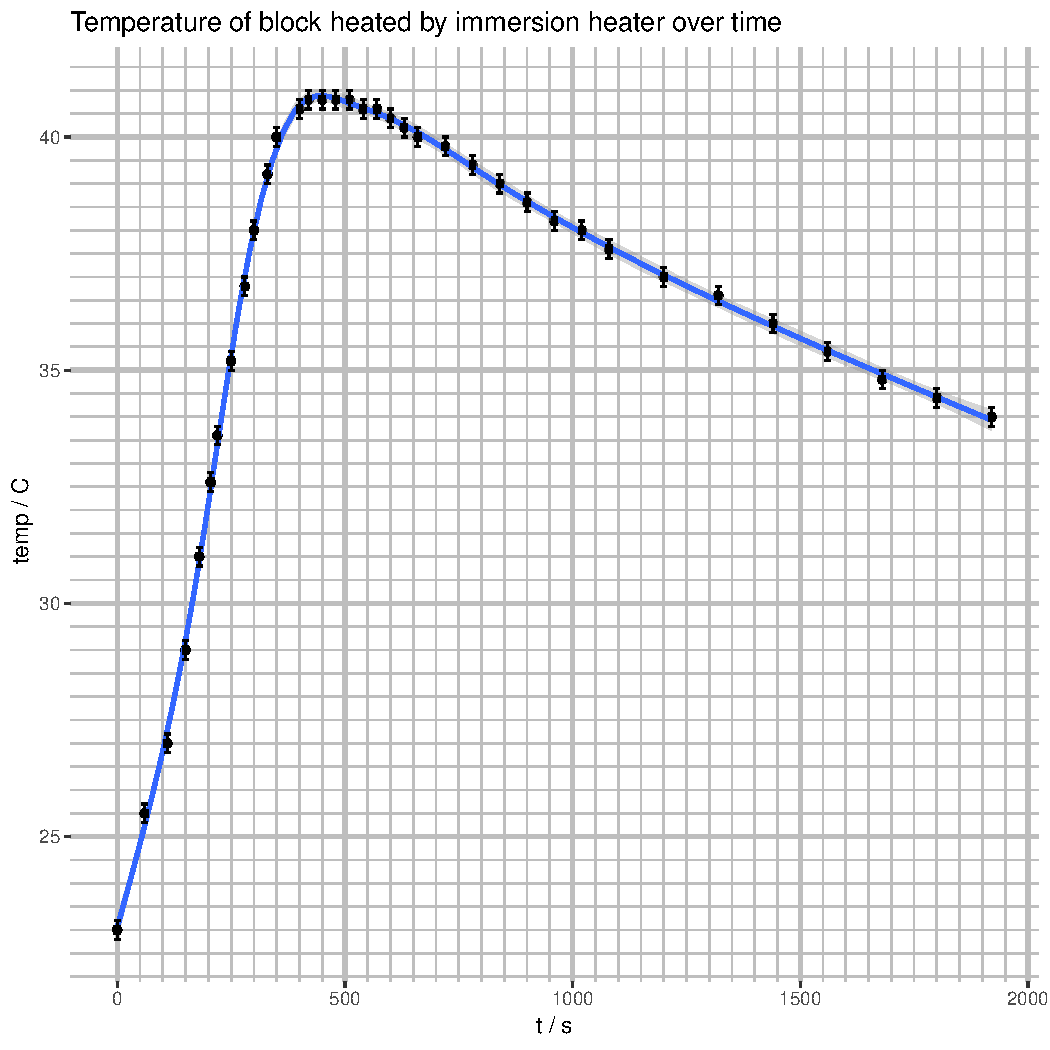
\includegraphics{Rplots.pdf}
\end{center}
\caption{Graph of temperature against time}\label{fig:graph}
\end{figure}

\begin{table}[h]
\begin{center}
\begin{tabular}{lS[table-format=1.7,table-align-text-post = false]}
$t_1$ & 446.8\,\si{s} \\
$t_2$ & 1473.2\,\si{s} \\
$A_1$ & 4537.0\,\si{\second\celsius} \\
$A_2$ & 21070.4\,\si{\second\celsius} \\
$\theta_{\text{corrected max}}$ & 42.3\,\si{\celsius} \\
$\theta_{\text{start}}$ & 23.0\,\si{\celsius} \\
$t_{\text{heat}}$ & 210.0\,\si{s} \\
$c$ & 0.45\,\si{\joule \per \gram} \\
\end{tabular}
\end{center}
\caption{Intermediate values in the calculation of $c$}\label{tab:values}
\end{table}

\nocite{*}
\bibliographystyle{agsm}
\bibliography{sources}

\end{document}
